%************************************************
\section{Black-box Analysis}\label{ch:Blackbox}
%************************************************
When developing a software system, it often happens that we need different frameworks or other systems to develop ours.
While it would be possible to develop these systems ourselves, in most cases this is inefficient and slows down the release of our system.
To speed up this process, we can use other systems that are already available to us, this however introduces us to the issue whether the system 
also fulfills our needs besides functionality, for example performance. 

For this purpose, we can perform a black-box analysis of the system. 
A black-box analysis is conceptually simple, given a configurable system, we select a configuration that contains the feature we are interested in. 
We run the system with different configuration containing the features we are interested in,
during execution we measure the non-functional properties we can observe.
Next, we use these measurements to build a performance-influcence model, that becomes more accurate as the number of unique configurations measured increases. 
Since it is not feasible to measure all possible configuration, we use our model to predict the time it takes to run a configuration
having to run the configuration on the system.


\begin{figure}[h]
    \centering
    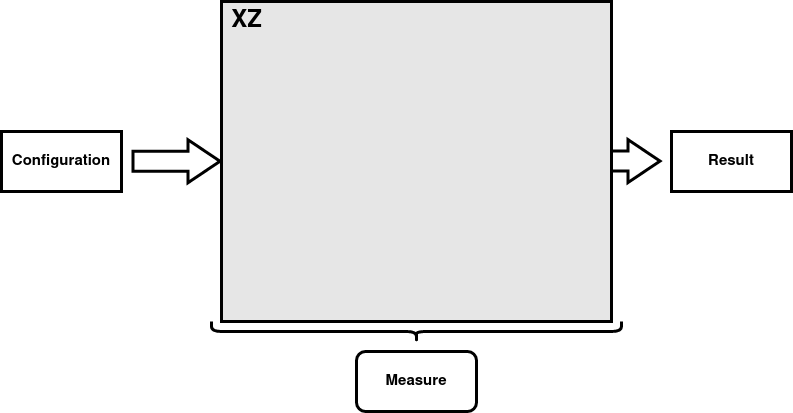
\includegraphics[scale=0.6]{gfx/BlackBoxXZ.png}
    \caption{A Black-box Version of xz}
    \label{fig:BBxz}
\end{figure}

As an example for a black-box analysis we modify xz from \ref{fig:xz}. To perform a black-box analysis we feed xz with the different configuration that
contain the features we choose to measure. Now, for each configuration we observe the properties we are interested in, such as time spend during the 
execution of the system, how xz produces these result we cannot tell. After repeating this process multiple time we use all the measurements collected to 
build a performance-influcence model that represents xz.

\subsection{Disadvantages of black-box model}
Even though a black-box analysis is simple in nature, it faces two major challenges, namely combinatorial explosion and collinear features, both need to be
handled carefully in order to build an accurate performance-influence model.

\paragraph{Combinatorial Explosion}
One of the larger problems we face when using black-box models is the issue of combinatorial explosion, 
which refers to the effect that when features increase linearly, the number of possible configuration and thus system variants,
increase exponentially \cite{Combinatorial-explosion}.

Suppose we have a configurable system where each feature is a binary option that you can either select or deselect. We also define 
that in this system each feature is completely independent of another, (i.e. the system has no constraints and selecting or deselecting a featureMuss
has no effect on other features). The number of unique configurations this system can produce is $2^n$, where $2$ refers to
the type of feature options allowed, binary in our case and $n$ denotes the number of features. 

Here lies the problem, all these different features might interact with each other in different ways, and for very small systems,
we can certainly brute-force our way by benchmarking all possible configuration, however this does not scale, it is already not feasible for 
larger systems. As an example, the Linux kernel contains 10000 different features \cite{Linux-Kernel}, for reference it is estimated that the universe
contains about $10^{79}$ atoms, which is still less than the variants of a system with 263 features, it is already impossible to use brute-force to analyze
such as system, let alone the Linux kernel.

For this reason, we cannot fully explore the entire configuration space 
and therefore need to select a subset that represent the system with a high accuracy. To do that state of the art black-box model use sampling
strategies to find a suitable subset, such as, pair-wise sampling, most-enabled-disabled and random sampling.

\paragraph{Multicollinear Features}\label{ColinearF}
We have already mentioned that features that do not influence each other are called independent features, but configurable systems are composed
of not only independent features. If there is a dependence between more than two features, we call these features multicollinear.

The reason why multicollinearity is a problem in a black-box analysis is
that we can only observe nun-functional properties during execution and are unable to correctly assign the influence of each feature
on the system. One way multicollinearity is introduced into a system is by using alternative groups, since the selection of a feature in the
alternative group depends on which options are chosen by the other features in that group. \cite{Multicollinearity}
\pagebreak

\begin{table}[h]
    \centering
    \begin{tabular}{llllll}
    \hline
    Base & A & B & C &  & $\bm{\Pi(*)}$ \\ \hline
    1 & 1 & 0 & 0 &  & $\mathbf{5}$  \\
    1 & 0 & 1 & 0 &  & $\mathbf{10}$  \\  
    1 & 0 & 0 & 1 &  & $\mathbf{15}$  \\\hline
    \end{tabular}  
    \caption{Configuration example illustrating multicollinearity in an alternative group}\label{tab:alternative}
\end{table}

Now consider the example of \ref{tab:alternative}, where we see a configuration example that contains multicollinear features due to an alternative group.
The example contains a Base feature and 3 features for an alternative A, B, and C, which means only one these 3 features can be selected for each
configuration.
This now clearly shows the dependency between these features, because for feature C to be selected, B and C needs to be deselected, which means
$C = 1 - B - C$ needs to be satisfied. 

\begin{align*}
    \Pi(c) &= 0 + 5 \cdot c(A) + 10\cdot c(B) + 20\cdot c(C) \\
    \Pi(c) &= 5 + 10 \cdot c(A) + 5\cdot c(B) + 20\cdot c(C) \\
    \Pi(c) &= 8 + 20 \cdot c(A) + 10\cdot c(B) + 7\cdot c(C) \\
\end{align*}

This, leads us to multiple performance-influcence model that are accurate regarding each measurement, but when we
compare them state completely different things. 
The problem here is that since one child of the alternative must be selected, but the other are deselected, we cannot correctly infer the influence
all features has on to the system as we can see in our example base is attributed $0$, $5$ and $8$. 
These values of base or the selected feature can be set in any ratio, as long as the sum of the two is equal to the time we measured.

A different way multicollinearity is introduced into the system is when we have features that are mandatory or connected by a condition. 
If we have features that are mandatory, we are unable to distinguish these features with our black-box analysis because they are always selected
together, we are unable to determine the extent to which each feature influences the system. \cite{Multicollinearity}

\begin{algorithm}[h]
    \caption{Equivalence \label{alg:Colinear}}
    \begin{algorithmic}[1]

    \If{$(c \textit{ and }  \lnot d) or (\lnot c \textit{ and } d)$} 
        \State $c,d \gets False$
    \EndIf

    \end{algorithmic}
    \end{algorithm}

Extending the example code from \ref{alg:performanceExample} with an additional condition where $C \equiv D$ holds, so that 
either C or D can be selected without the other, we insert the code snippet \ref{alg:Colinear} after \ref{alg:code_insertion}.

Now, if we select a configuration c containing the features \{\{A\}, \{B\}, \{C\}\} we get multiple {\perfInfluenceModel}s:

\begin{align*}
    \Pi_1(c) &= 1 + 1\cdot c(C) + 1 \cdot c(D) + 1\cdot c(C) \cdot c(D) \\
    \Pi_2(c) &= 1 + 0\cdot c(C) + 0 \cdot c(D) + 3\cdot c(C) \cdot c(D) \\
    \Pi_3(c) &= 1 + 1\cdot c(C) + 2 \cdot c(D) + 0\cdot c(C) \cdot c(D) \\
\end{align*}

All the {\perfInfluenceModel}s are accurate with respect to the measurements, but assign different values to each feature. 
In $\Pi_1(c)$ and $\Pi_2(c)$, all features are assigned different values from what we would expect when looking at \ref{alg:performanceExample},
while the \perfInfluenceModel of $\Pi_C(c)$ assigns the expected values.

\subsection{Selecting the configuration space}
Software products keep improving and to add more functionality they increase the number of optional features as well, this dramatically increases 
the configuration space as well, however it was already shown by Tianyin Xu et. al. \cite{TooManyKnobs} that not all features are equally important and that up to
54,1\% of features are rarely set by any users.

We take advantage of this knowledge to deal with the problem of combinatorial explosion, by using our domain knowledge to extract the most important
features we are interested in. This also helps us to mitigate the influence of multicollinear features, since we are selecting which feature to add
into our configuration space we can assure to keep the dependency between our selected features to a minimum.

\subsection{Collecting data}
After deciding which features interest us we can now move on to how we collect our data that we can afterwards use to build a \perfInfluenceModel.

Since, we use a black-box analysis our methods are quite limited, like depicted in \ref{fig:BBxz} we are not able to inspect what the system does 
in detail and are limited to the properties that we can observe from our outside view. In this case we can measure non-functional properties
such as time to completion, energy consumption, memory usage, computational resources used, basically every value we can observe by looking at the
machine that runs the system. If it is possible measurements should be repeated at least 30 time to reduce measurement noise during execution 
\cite{SampleSize}.


\subsection{Creating a Performance-Influence Model using Multiple Linear Regression}
After we collected all our measurements we use them to build our \perfInfluenceModel of the system. 

To build the model there are different
approaches available, one popular one is using neural networks, however these come with major disadvantages such that the model itself 
loses its explainability and is are commonly not comprehendable, due to these reasons we have decided to use multiple linear regression.

There are a multitude of reasons why we use multiple linear regression, one is that compared to a neural network the linear model we 
derive is easy to understand and interpretable for us humans, it also it is already very similar to the structure of a \perfInfluenceModel.

We use the following formula of linear regression for matrices\cite{Linear-Regression-Performance}:

\begin{align*}\label{formula:linReg}
    Y &= \beta_0 + \beta_1 x_1 + \beta_2 x_2 ... \beta_n x_n + \epsilon   \\
    Y &= X \beta + \epsilon \\\\
    Y &= \textit{Dependent variable}\\
    X &= \textit{Independent variable}\\
    \beta &= \textit{Regression coefficient}\\
    \epsilon &= \textit{Error}\\
\end{align*}


Where $y$ is called dependent variable and $X$ is called independent variable, $y$ in our case is a vector with n elements containing
the output of our black-box model, i.e. the time measurement generated for each feature configuration in our feature set. What we
are interested in are the values of the coefficients $\beta$, since they quantify the influence of each feature or feature interaction
on to the whole system. In addition, $\beta_0$ denotes the intercept, which for us represents the influence of the base code, meaning
the part of the code that gets executed regardless of the selected feature configuration.

To accommodate feature interactions in this linear model, we add a term for each interaction we want to include, for example,
if we are in the interaction between feature $x_i$ and $x_j$ we add the term $\beta_k x_i x_j$. 
Our independent variable $X$ is an $n \times m$ matrix, where $n$ is the number of configurations used and $m$ the number of configurations
in our set of configurations $\mid \mathcal{C} \mid$.

The value of each feature in the matrix is either $1$ if the feature is selected, or $0$ if it is not. If we have numerical features with $l$
different options, we split this features into $l$ binary features and encode them as an alternative group in our feature model.

For all our measurements have a possible error represented by $\epsilon$. \cite{Linear-Regression}

\subsubsection{Least Ordinary Squares}
Now that we have seen the overall formula of linear regression and what the different components represent we still need to find out 
how to calculate the regression coefficient $\beta$, the values that tell us the influence of each feature. 

For this purpose we use the least ordinary square estimator, which is optimal for the class of linear unbiased estimator, 
however it is unreliable if the independent variables $X$ contain a high degree of multicollinearity.
The principal behind least ordinary squares is to minimize the sum of the squared residuals, where the residual is the difference between
the predicted value of the estimator and the actual value. \cite{Linear-Regression}




To calculate the values $\beta$ we use the estimator least odinary squares

\paragraph{Variance inflation factor}
